%---Packages---%
\documentclass[a4paper,11pt]{article}
\usepackage[left=2.5cm,top=2cm,right=2cm,nohead]{geometry}
\usepackage[french]{babel}
\usepackage[T1]{fontenc}
\usepackage[utf8]{inputenc} 
\usepackage{graphicx}
\usepackage{float}
\usepackage{amsmath}
\usepackage{amsfonts}
\usepackage{amssymb}
\usepackage{listings}
\usepackage{mdwlist}
\usepackage[usenames,dvipsnames]{color}
\usepackage[stable]{footmisc}%To include footnotes in 'section' parts
\usepackage{hyperref}
\usepackage{setspace}
\usepackage{eurosym}
\usepackage[section]{algorithm} % [section] is use to define the numbering mode
\usepackage{algorithmic} 

%---Insertion de code---%
\definecolor{lightgray}{gray}{0.95}


\lstset
{           
backgroundcolor=\color{lightgray},
keywordstyle=\color{Red}\bfseries,
ndkeywordstyle=\color{darkgray}\bfseries,
commentstyle=\color{Green},
stringstyle=\color{Orange},
basicstyle=\footnotesize,       % the size of the fonts that are used for the code
numbers=left,                   % where to put the line-numbers
numberstyle=\footnotesize,      % the size of the fonts that are used for the line-numbers
stepnumber=2,                   % the step between two line-numbers. If it's 1 each line will be numbered 
numbersep=5pt,                  % how far the line-numbers are from the code
showspaces=false,               % show spaces adding particular underscores
showstringspaces=false,         % underline spaces within strings
showtabs=false,                 % show tabs within strings adding particular underscores
tabsize=2,	                % sets default tabsize to 2 spaces
captionpos=b,                   % sets the caption-position to bottom
breaklines=true,                % sets automatic line breaking
breakatwhitespace=false,        % sets if automatic breaks should only happen at whitespace
title=\lstname,                 % show the filename of files included with \lstinputlisting & 
escapeinside={\%*}{*)},         % if you want to add a comment within your code
morekeywords={*,...}            % if you want to add more keywords to the set
extendedchars=true
}

%---Liens---%
\hypersetup{
unicode=false,          % non-Latin characters in Acrobat’s bookmarks
pdftoolbar=true,        % show Acrobat’s toolbar?
pdfmenubar=true,        % show Acrobat’s menu?
pdffitwindow=false,     % window fit to page when opened
pdfstartview={FitH},    % fits the width of the page to the window
pdftitle={Projet AGGP - Synthèse des articles},    % title
pdfauthor={Balthazar Rouberol, Anthony Tschirhard, Marion Poirel, Marie Paturel},     % author
pdfsubject={Projet AGGP - Dossier d'init},   % subject of the document
pdfcreator={Balthazar Rouberol, Anthony Tschirhard, Marion Poirel, Marie Paturel},   % creator of the document
pdfkeywords={Réseaux biologiques, Réseaux, AlgoGen}, % list of keywords
pdfnewwindow=true,      % links in new window
colorlinks=true,       % false: boxed links; true: colored links
linkcolor=black,          % color of internal links
citecolor=black,        % color of links to bibliography
filecolor=white,      % color of file links
urlcolor= NavyBlue,           % color of external links
bookmarks=true,% show bookmarks bar?
bookmarksopen=false,
bookmarksnumbered = false      
}%



\title{Projet AGGP - Synthèse des articles}

\begin{document}
\maketitle 

\section{Mesures possibles sur réseaux}

\paragraph*{Degré d'un noeud : $k$\\}
Représente le nombre de connexions branchées sur un noeud. 

\paragraph*{Degré moyen d'un graphe : $<k>$\\}
Représente le nombre moyen de connexions branchées sur un noeud dans le graphe. 

\paragraph*{Distribution des degrés : $P(k)$\\}
La distribution des degrés des noeuds du graphe donne des informations sur la nature du graphe : scale-free, random\ldots

\paragraph*{"Degree exponent" : $\gamma$\\}
Ce paramètre n'a de sens que dans le cas de scale-free networks. Il traduit le rôle des hubs dans le réseau.

\paragraph*{Plus petit chemin : $l$\\} 
Le plus petit chemin qui relie deux noeuds. Attention, dans le cas de graphes orientés, il est probable que $l_{AB} \neq l_{BA}$.

\paragraph*{Plus petit chemin moyen : $<l>$\\}
Moyenne des plus petits chemins qui relient deux à deux tous les noeuds du graphe. $<l>$ traduit la navigabilité du graphe : plus $<l>$ est petit, plus le chemin entre deux points du graphe est court. 

\paragraph*{Coeffcient de clustering : $C_I$\\}
Nombre de "triangles" ABI passant par le noeud I, où A et B représentent deux noeuds du graphe. $C_i = \dfrac{2n_i}{k(k-1)}$, avec $n_I$ le nombre de liens reliant les $k$ voisins de I. $C$ est la signature d'une potentielle modularité du graphe.

\paragraph*{Coefficient de clustering moyen : $<C>$\\}
Moyenne des $<C_I>$.

\paragraph*{Distribution des coefficients de clustering : $P(C)$\\}
Traduit le caractère hiérarchique du réseau : $C(k) \sim k^{-1}$

\medskip
\raggedright
\textbf{\textcolor{red}{Important : }}\\
$<k>, <l>, <C>$ dépendent du nombre de noeuds et de liens $(N,L)$ du graphe, alors que $P(k)$ et $C(k)$ n'en sont pas dépendant. Ces deux derniers paramètres permettent de caractériser le réseau : scale-free, random\ldots

\section{Réseau aléatoire}
On construit un réseau aléatoire en connectant un nombre fixe N de noeuds de façon aléatoire.
On sait que dans un réseau aléatoire, $P(k)$ suit une distribution de Poisson. \\
Les réseaux aléatoires ne peuvent pas expliquer les propriétés topologiques des réseaux biologiques. Dans de tels réseaux, $<l> = log(N)$ : propriété de "petit monde". 

\section{Scale free networks}
Dans ce type de réseau, on prend en compte la présence de noeuds très fortement branchés aux autres noeuds du graphes. De tels noeuds sont appelés des \textbf{hubs}. 

\medskip
Exemple: 
\begin{itemize}
	\item sur internet : Twitter, Google, Youtube, Facebook,\ldots
	\item dans un réseau métabolique : ATP, ADN$_{pol}$, \ldots
\end{itemize}

\medskip
La présence de ces hubs bouleverse la distribution de $<P(k)>$. On a alors $P(k) \sim k^{-\gamma}$ (\textbf{loi de puissance}), avec $\gamma$ degree exponent, traduisant le rôles des hubs dans le réseau.

\medskip
La valeur de $\gamma$ est primordiale pour caractériser le réseau :
\begin{itemize}
	\item $\gamma$ > 3 : pas de hubs dans le réseau. Ce n'est pas un scale-free,
	\item $2 < \gamma < 3$ \textbf{(le cas de la majorité des réseaux biologiques)}: hiérarchie de hubs et $<l>$ = log(log(N)) : propriété de (très) petit monde,
	\item $\gamma = 2$ : présence d'un très gros hub.\medskip
\end{itemize}

On a trouvé que la majorité des données sont le mieux fittées si $\gamma \simeq 2.1$. Les réseaux cellulaires, métaboliques, sociaux \ldots sont scale-free.

\section{Comparaison des types de réseaux}
\begin{figure}[h!]
	\raggedleft
	\begin{minipage}{0.60\linewidth}
		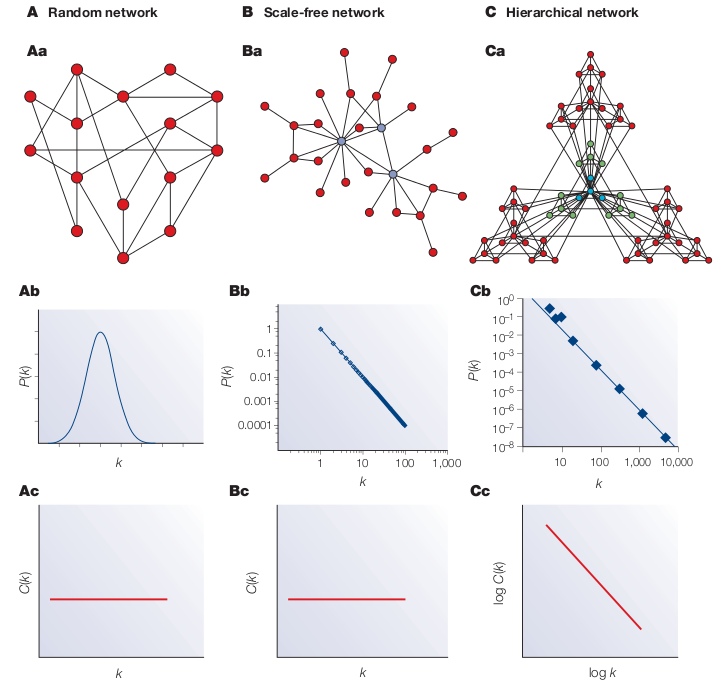
\includegraphics[width=\linewidth]{Nwk.png}
		\caption{Random (A), scale-free (B), hierarchic (C)}
	\end{minipage}
	\raggedright
	\begin{minipage}{0.35\linewidth}
		
		\textbf{Réseaux aléatoires},\\ $<P(k)>_{max} \simeq <k>$.\\ Si $p$ est la probabilité de connecter une paire de noeuds, on a environ $\dfrac{pN(N-1)}{2}$ liens. \\$C(k)$ indépendant de $k$.
		
		\medskip
		\textbf{Scale free networks} :\\
		Les noeuds bleus sont statistiquement plus connectés que dans un réseau aléatoire : ce sont des hubs.\\
		$<l>$ = log(log(N)) : effet des hubs.
		
		\medskip
		\textbf{Hierarchical networks}:\\
		Combinaisons de clusters générant des réseaux hiérarchiques.
		
	\end{minipage}			
\end{figure}

\section{Propriétés de réseaux biologiques}
Un réseau biologique doit (si je ne me trompe pas) valider les conditions suivantes : 
\begin{enumerate}	
	\item $<P(k)> \sim k^{-\gamma}$ (Power law) avec $2<\gamma<3$,
	\item valider une propriété de petit monde (inclus dans la 1?),
	\item avoir une forte resistance ($\simeq$80\% des nodes sont "éjectables") (inclus dans la 1?)
	\item formation de cliques/modules : contradictoire avec la propriété de petit monde => TRADE-OFF à déterminer.
\end{enumerate}
\end{document}
